\documentclass[11 pt]{article}

\setlength{\oddsidemargin}{-.35in}
%\setlength{\evensidemargin}{-.5in}
\setlength{\textwidth}{7.0in}
\setlength{\topmargin}{-0.95in}
\setlength{\textheight}{10.0in}

\usepackage{graphicx}
\usepackage{latexsym}
\usepackage{amsfonts}
\usepackage{amsmath}
\usepackage{amsthm}

\usepackage[T1]{fontenc}
%\usepackage{baskervald}
%\usepackage[bigdelims,vvarbb]{newtxmath} 

\usepackage{hyperref} 
\hypersetup{colorlinks=true, linkcolor=blue,  anchorcolor=blue,  
citecolor=blue, filecolor=blue, menucolor=blue, pagecolor=blue,  
urlcolor=blue}

\pagestyle{empty}

%\renewcommand{\baselinestretch}{1.5}

\begin{document}

\noindent MTH 201: Calculus \ \ \ Checkpoint 2 (SAMPLE) \hfill Talbert \\

\noindent {\bfseries Directions:} Choose \emph{only the Learning Targets you are ready to check}. For each of those, give a complete solution that shows all relevant work and gives clear, logical explanations of your reasoning. Please: 

\begin{itemize}
    \item Do NOT put any work on this form. 
    \item When done with one Learning Target, start a new page for each additional one; don't place work for multiple learning targets on the same page. 
    \item Clearly indicate which Learning Target you are attempting at the beginning of its solution. 
    \item \textbf{Unless the problem statement explicitly states that only the answer is required, you must show all relevant work and explain your reasoning in clear, logical terms. Your grade will be based on the quality of your reasoning, not only the correctness of the answer.}
    \item When done, put all your work in order (use the same ordering of Learning Targets as you see on this form). 
    \item When done, \textbf{scan your work to a clear, black-and-white PDF} of size less than 100 MB, and \textbf{upload the PDF's to the indicated Assignment on Blackboard, in the Checkpoints area}. 
    \item DO NOT simply take a photo of your work; use a scanning app or scanner. Also DO NOT email your work to the professor; upload it to Blackboard. Work that consists of photos (not scans) and work received by email (unless Blackboard is inaccessible) will not be graded and may be given a grade of "N" for repeat instances. 
\end{itemize}

\noindent \hrulefill

\begin{description}

\item[Learning Target F.1: ] \textit{I can find the average rate of change of a function on an interval.}

\begin{enumerate}
    \item Let $f(x) = 2^x + x$. Find the average rate of change in $f$ on the intervals $[0,1]$ and $[-1, -1.1]$. 
    \item Let $g(x)$ be given by the graph below. Find the average rate of change in $g$ on the intervals $[-4,0]$ and $[0,1]$. 
    \begin{center}
        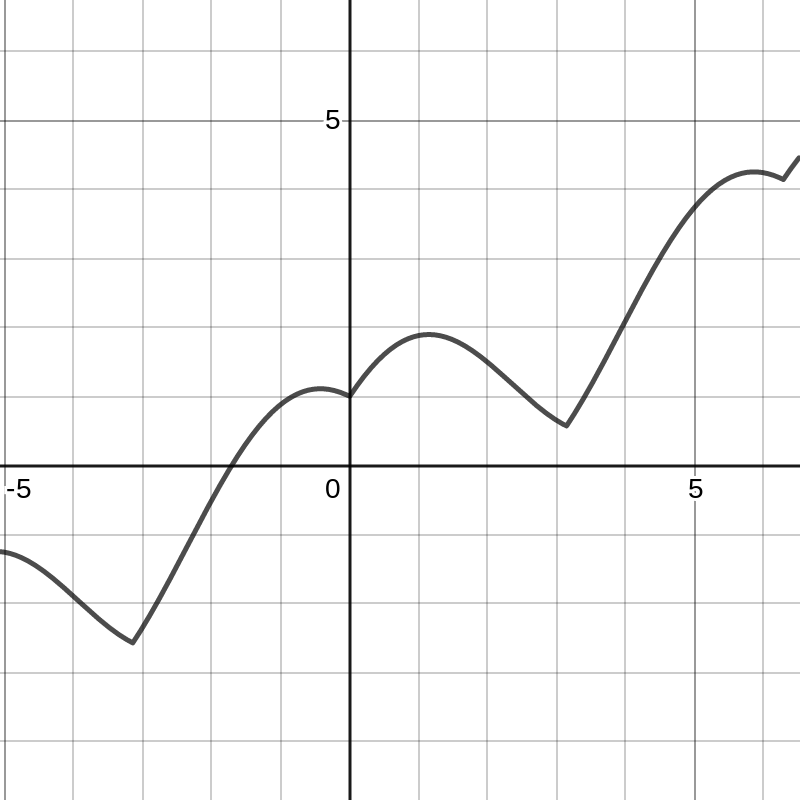
\includegraphics[width=2in]{c2p2-sample-f1.png}
    \end{center}
\end{enumerate}

\vfill \eject

\item[Learning Target L.1 (\textbf{Core}): ] \textit{I can find the limit of a function at a point using numerical, graphical, and algebraic methods.} 

\begin{enumerate}
    \item Complete the table of values below using the function $f(x) = \dfrac{x^2 + 3x -10}{x-2}$. Then state the value of $\lim_{x \to 5} f(x)$ and explain your reasoning. 
    
        \begin{tabular}{l|l|l|l|l|l|l}
        $x$    & 1.5 & 1.9 & 1.99 & 2.01 & 2.1 & 2.5 \\ \hline
        $f(x)$ &     &     &      &      &     &    
        \end{tabular}
        
    \item Using only algebra (no graphs or tables), evaluate $\lim_{x \to 5}\dfrac{x^2 - 4x - 5}{x-5} $.
    \item The function $h(x)$ is shown below. State the value of $\lim_{x \to 1} h(x)$ and explain your reasoning.
    \begin{center}
        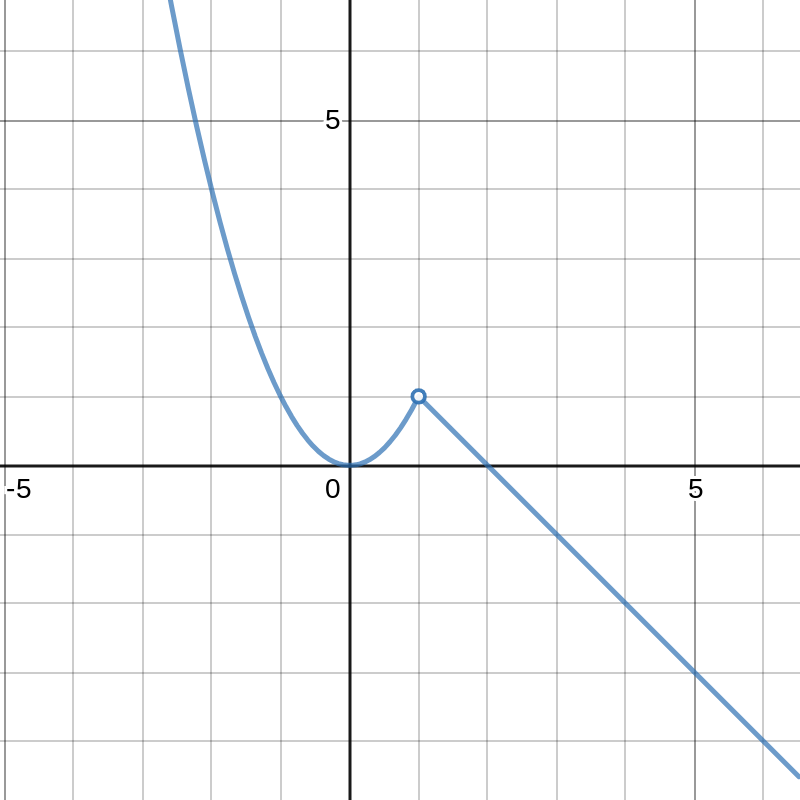
\includegraphics[width=2in]{c2p2-sample-l1.png}
    \end{center}
    
\end{enumerate}

\item[Learning Target D.1 (\textbf{Core}):] \textit{I can find the derivative of a function, both at a point and as a function, using the definition of the derivative.}


\begin{enumerate}
    \item Let $f(x) = x^2 - 4x - 5$. Use the definition of the derivative to compute the value of $f'(3)$. 
    \item Also using $f(x) = x^2 - 4x - 5$, use the definition of the derivative function to find a formula for $f'(x)$. 
\end{enumerate}

\end{description}


\end{document}
